%!TEX ROOT=main.tex


\chapter{Personal development domain}\label{ch:personal-development-domain}


This section will introduce the reader to the domain of personal development.
Justification of the idea behind the application will also be presented here.

%Use empirical statements


\section{Definition of personal development}\label{sec:definition-of-personal-development}

In order to create helpful application, it is crucial to build it based on principles and ideas of personal development.
Familiarisation with these will start from the definition of personal development and with Maslow's hierarchy of needs in particular.

\begin{figure}[h]
    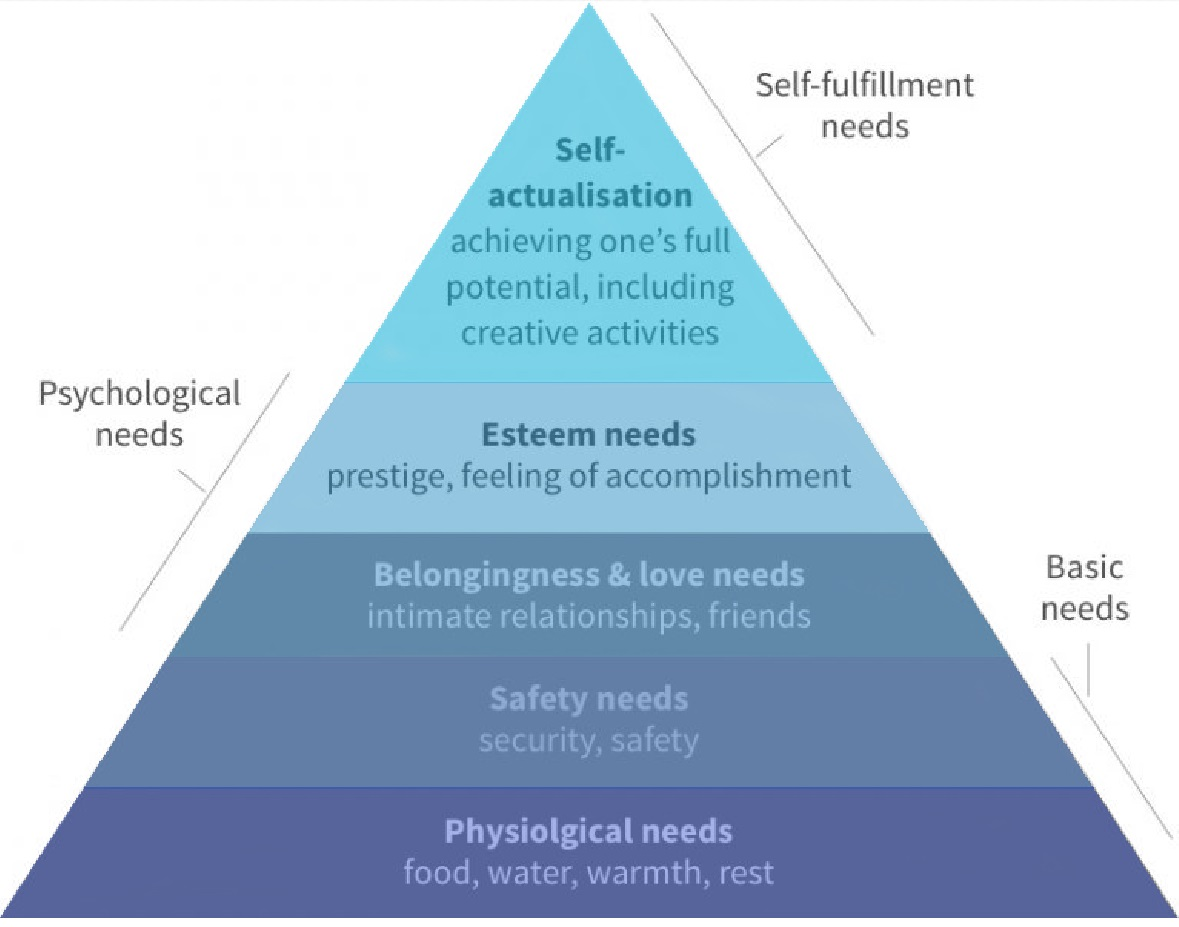
\includegraphics[width=0.75\textwidth]{images/maslows.jpg}
    \caption{Maslow's Hierarchy of Needs ~\cite{maslow-pyramid}}
    \label{fig:maslow-pyramid}
\end{figure}

The pyramid shown in figure~\ref{fig:maslow-pyramid} might be familiar to the reader.
It was first introduced by A. Maslow in 1943~\cite{maslow-motivation}.
This pyramid represents the hierarchy of common human needs.
It may be presumed, that a person has satisfied lower levels before beginning to satisfy the higher ones.
Going from the bottom to the top, the first two levels are basic needs that every person needs the most.
The following two levels are psychological needs, these come after physical ones.
At the top of the pyramid there is a need for ~\textit{self-actualisation}.
Maslow described it as restlessness that often develops even with satisfied needs.
Self-actualisation refers to the desire of reaching one's full potential and could be considered as the goal and motivator for the process of personal development.
As pyramid contains highly relatable needs and was popularized in modern culture, it is safe to assume that described needs will be known to the reader.

\textit{Personal development} is the set of activities aimed at enhancement of employability, improvement of quality of life and raising one's confidence ~\cite{what-is-personal-development}.
Motivation for personal development comes from the need for self-actualisation and thereby makes it a natural and relatable feeling.
Five following steps should be considered when managing one's personal development, hence should be attended in the application:
personal vision development, personal development planning, starting the improvement process, recording personal development, reviewing and revisiting personal development plans.

\textit{Development of personal vision} means having an idea of what person wants to become in the future.
Decision making cannot be helped by the application, because of highly personal and case-specific nature of the process.
On the other hand, results of those decisions will be managed by application, those will be the source of goals.
One might consider goals as personal projects.
Due to simplicity of this action on behalf of the application, new goal creation has also stay simple and require the lowest possible amount of mandatory fields.

After personal vision decisions comes personal ~\textit{development planning}.
This step is optional, but crucial for long-term goals with a large amount of different milestones.
As an example, new skills learning might be more efficient with a plan rather than with an ad-hoc approach.
This also opens an opportunity for plans sharing feature.
Planning would obsolete in case of simple and repetitive activities, which emphasise the need for optionality of this feature.

The next step is to ~\textit{start the improvement process}.
Management of the process is outside of application scope.
The main aim is to motivate user and manage plans and results.
In order to cover this step in the application, it will be possible to set the beginning date of a goal at the point in the future.
Development planning also might benefit from that feature.

\textit{Recording personal development} is always a good idea when it comes to personal development as it makes the process measurable.
This is also one of the main points of the future application.
Activity record opens opportunity for both: data visualisation and social engagement.
%These records are also going to be used by the next step.

\textit{Reviewing and revisiting personal development plans} will allow one to learn more from past activities.
Another benefit is that the record might allow person to define a comfortable learning pace and improve future experience with the application and personal development in general.
For the application this means that there should be an easily accessible history of past goals and activities.

%Described steps ensure that data management flow of the application will correspond with the recommended way of approaching personal development.
Steps from above describe recommended approach to the personal development.
Those steps also define a data management flow of the application.
Domain-based approach will be able to provide better user experience when it comes to the process planning and data input.
%This approach also define which fields are mandatory and which are optional.



\section{Competitive attitude}\label{sec:competitive-attitude}

%https://www.frontiersin.org/articles/10.3389/fpsyg.2018.00779/full

%Regarding the personal-development competitive attitude (PDCA),
%the primary focus is on personal growth and on the enjoyment and mastery of the task in a competitive situation.
%The goal attainment and competition outcome (i.e., on winning) is important,
%but not at the expense of the derogation of other competitors (Ryckman et al., 1996).

